% \section*{Biographies of Authors}
\bigskip

\begin{wrapfigure}{l}{2cm}
    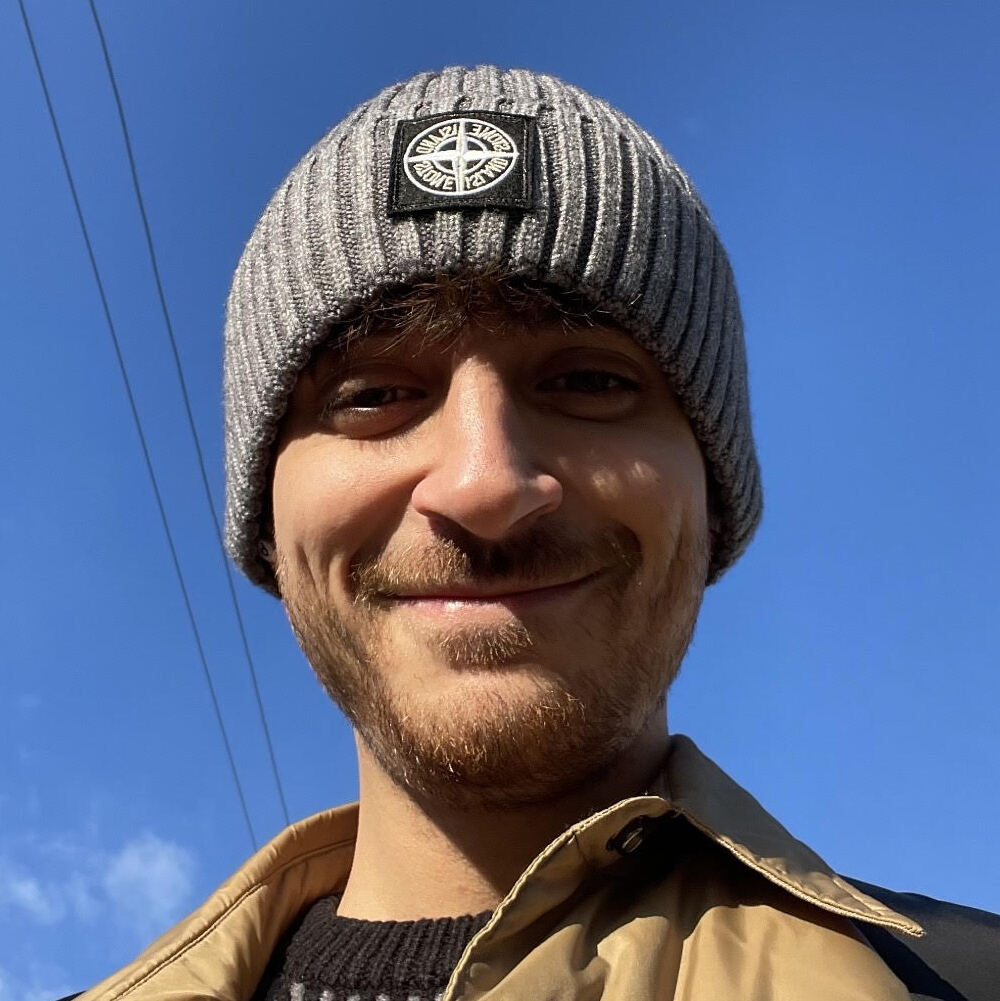
\includegraphics[width=2cm,keepaspectratio]{bios/federico}
\end{wrapfigure}\par
\noindent\textbf{Federico Bruzzone} is currently a Ph.D. student in Computer Science at Universit\`a degli Studi di Milano, Italy. He was born in 2000 and since he was a child he has been passionate about computer science and music. He got his bachelor degree in Musical Computer Science, the master degree in Computer Science and currently he is involved in the research activity of the ADAPT Lab. His main research interests are (but are not limited to) programming languages and compilers, software maintenance and evolution. For any question he can be contacted at \url{federico.bruzzone@unimi.it}.\smallskip

\begin{wrapfigure}{l}{2cm}
    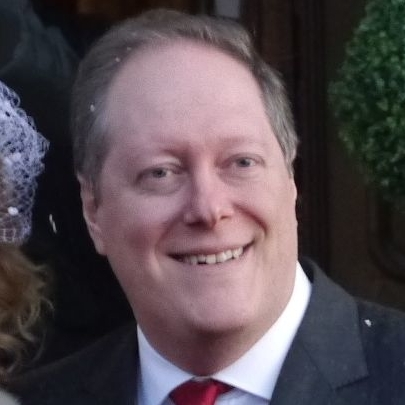
\includegraphics[width=2cm,keepaspectratio]{bios/walter}
\end{wrapfigure}\par
\noindent\textbf{Walter Cazzola} is currently a Full Professor in the Department of Computer Science of the Università degli Studi di Milano, Italy and the Chair of the ADAPT laboratory. Dr\@. Cazzola designed the mChaRM framework, @Java, [a]C\#, Blueprint programming languages and he is currently involved in the designing and development of the Neverlang language workbench. He also designed the JavAdaptor dynamic software updating framework and its front-end FiGA\@. He has written over 100 scientific papers. His research interests include (but are not limited to) software maintenance, evolution and comprehension, programming methodologies and languages. He served on the program committees or editorial boards of the most important conferences and journals about his research topics. He is associate editor for the Journal of Computer Languages published by Elsevier. More information about Dr\@. Cazzola and all his publications are available at \url{http://cazzola.di.unimi.it} and he can be contacted at \url{cazzola@di.unimi.it} for any question.\smallskip

